% !TEX spellcheck = en_US



% ~~~~~~~~~~~~~~~~~~~~~~~~~~~~~~~~~~~~~~~ V
% (NC) 2024Haluk Bingol
% github.com/halukbingol/LaTeX-Templates
%
% Licensees may copy, distribute, display, and perform the work and make derivative works 
% and remixes based on it only for non-commercial purposes. 
% ~~~~~~~~~~~~~~~~~~~~~~~~~~~~~~~~~~~~~~~ A




\documentclass{beamer}
	\usetheme{Dresden}
%	\usecolortheme{}
%	\useinnertheme{}
%	\useoutertheme{}
%	\setbeamertemplate{bibliography item}[text]
\usepackage{beamerthemesplit}
%\usecolortheme{default}
%\usecolortheme{structure}
%\usepackage{beamerthemesplit} // Activate for custom appearance




% ~~~~~~~~~~~~~~~~~~~~~~~~~~~~~~~~~~~~~~~ V HB lib
\usepackage{../hbcommon/hbdatastructures} 
\usepackage{../hbcommon/hbpresentation} 
% ~~~~~~~~~~~~~~~~~~~~~~~~~~~~~~~~~~~~~~~ A



% ~~~~~~~~~~~~~~~~~~~~~~~~~~~~~~~~~~~~~~~ V specific
	\usepackage[normalem]{ulem} %strikethroug
%	\sout{Hello World}

	\usepackage[ruled,vlined]{algorithm2e}

	\newcommand{\hDummy}{dummy}


%  ~~~~~~~~~~~~~~~~~~~~~~~~~~~~~~~~~~~~~~~ A




% ~~~~~~~~~~~~~~~~~~~~~~~~~~~~~~~~~~~~~~~ V
	\newcommand{\hAbs}[1]{\ensuremath{\left \lvert \, #1 \, \right \rvert} } % |x|
%	\newcommand{\hMean}[1]{\ensuremath{<\!\! #1 \!\!>}} % average
%	\newcommand{\hMean}[1]{\ensuremath{\overline{#1}}}
% ~~~~~~~~~~~~~~~~~~~~~~~~~~~~~~~~~~~~~~~ A


%: ==== HB Header Common Packages v20160423 ====V
	\usepackage[utf8]{inputenc} % To use Unicode characters
	\usepackage[iso]{datetime}
	%	\usepackage{etex}
	
%	\usepackage[a4paper]{geometry}
	
	\usepackage{xcolor}
	% black, blue, brown, cyan, darkgray, gray, green, lightgray, lime, 
	% magenta, olive, orange, pink, purple, red, teal, violet, white, yellow
%	\usepackage[colorlinks=true,linkcolor=red,urlcolor=blue,citecolor=red]%
%		{hyperref}
	\usepackage{graphicx,epstopdf}
	% \graphicspath{{fig}}
%	\graphicspath{{../common/figures/}}
	% \DeclareGraphicsExtensions{.pdf,.jpeg,.png,.eps}
	% \DeclareGraphicsRule{.tif}{png}{.png}%
	%	{`convert #1 `dirname #1`/`basename #1 .tif`.png}
%	\usepackage{subfigure}
%\usepackage{subfig}
%\usepackage{subcaption}
% ~~~~~~~~~~~~~~~~~~~~~~~~~~~~~~~~~~~~~~~ V HB Header Common Packages v20160423 




% ~~~~~~~~~~~~~~~~~~~~~~~~~~~~~~~~~~~~~~~ V
\title{
	cis112\\
	Stack
}

\author[Bingol]{Haluk O. Bingol}

\institute{
	Faculty of Computer and Information Sciences\\
	Yeditepe University
}

%\date{
%	cis112\\ 
%	Yeditepe University, 2024-02-25
%}
\date{
	{\tiny \hbTimeStamp}
}
% ~~~~~~~~~~~~~~~~~~~~~~~~~~~~~~~~~~~~~~~ A



\begin{document}
% ~~~~~~~~~~~~~~~~~~~~~~~~~~~~~~~~~~~~~~~ 




% ~~~~~~~~~~~~~~~~~~~~~~~~~~~~~~~~~~~~~~~ V Title
\frame{\titlepage}
% ~~~~~~~~~~~~~~~~~~~~~~~~~~~~~~~~~~~~~~~ A 




% ~~~~~~~~~~~~~~~~~~~~~~~~~~~~~~~~~~~~~~~ V Content
\begin{frame}\frametitle{Content}
	\begin{columns}[T]
	\begin{column}{.5\linewidth}   
	    	\tableofcontents
	\end{column}
	\begin{column}{.5\linewidth}
%		\vspace{1cm}
		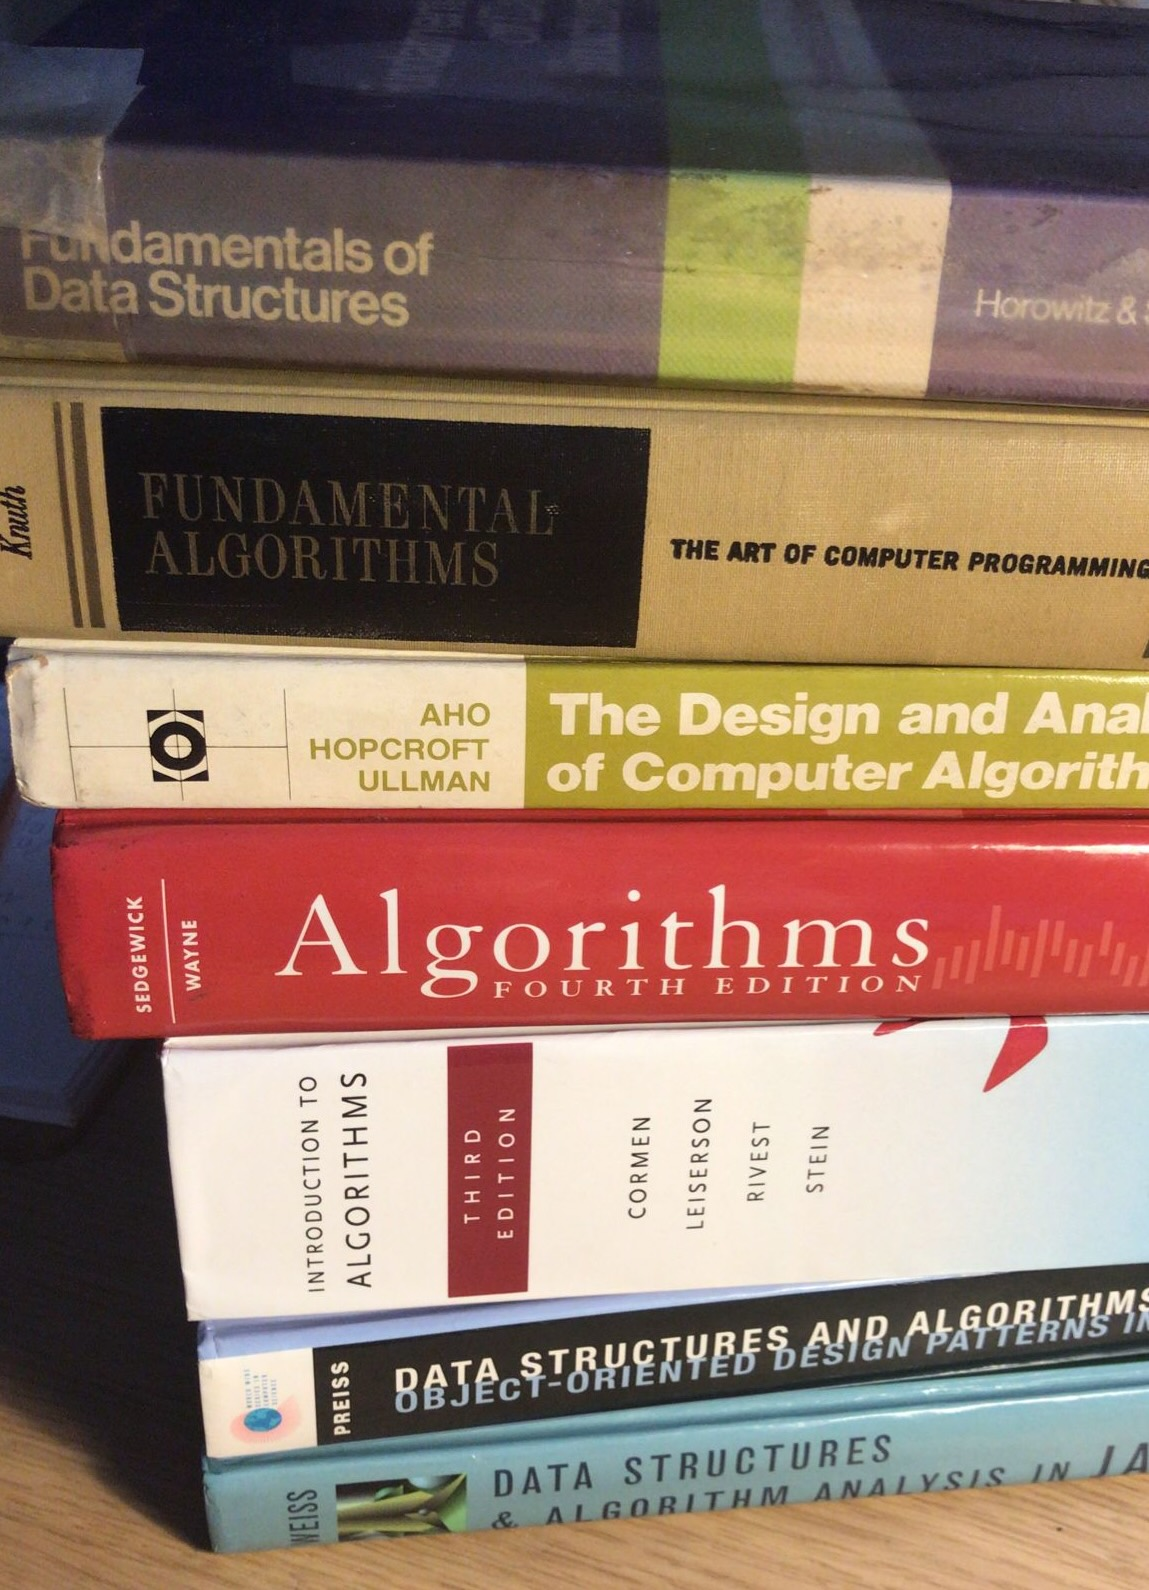
\includegraphics[width=.8\columnwidth]
			{fig-stackBooks.jpg}\\
		{\small Stack of books}
	\end{column}
	\end{columns}
\end{frame}
% ~~~~~~~~~~~~~~~~~~~~~~~~~~~~~~~~~~~~~~~ A




% ~~~~~~~~~~~~~~~~~~~~~~~~~~~~~~~~~~~~~~ V
\hSection{Motivation}{}{}
% ~~~~~~~~~~~~~~~~~~~~~~~~~~~~~~~~~~~~~~ A




% ~~~~~~~~~~~~~~~~~~~~~~~~~~~~~~~~~~~~~~ V
\begin{frame}\frametitle{Motivation}

How does 

	\begin{itemize}

		\item 
		browser keep track of previous visited pages?

		\item 
		a text editor handle undo operations?

		\item 
		compiler check if the parentheses balanced?
		\begin{itemize}
			
			\item 
			Balanced: (),  (()),  ()(), (()((())))
			
			\item 
			Unbalanced: )(,  (())),  ())(), ((()((())))
			
		\end{itemize}

		\item 
		evaluate expression
		\begin{itemize}
			
			\item 
			1 + 2 * 3
			
		\end{itemize}
	\end{itemize}
\end{frame}
% ~~~~~~~~~~~~~~~~~~~~~~~~~~~~~~~~~~~~~~ A




% ~~~~~~~~~~~~~~~~~~~~~~~~~~~~~~~~~~~~~~ V
\hSection{Case: Browser visiting pages}{}{}
% ~~~~~~~~~~~~~~~~~~~~~~~~~~~~~~~~~~~~~~ A




% ~~~~~~~~~~~~~~~~~~~~~~~~~~~~~~~~~~~~~~ V
\begin{frame}\frametitle{Case: Browser visiting pages}

\begingroup
\setlength{\tabcolsep}{3pt}
\renewcommand{\arraystretch}{.1}
\begin{center}
\begin{tabular}{l l l}

	%
	\textbf{Visit page} &\textbf{Page seen}
	&\textbf{History}\\
	%
	\pause
	A &A
	&\begin{tikzpicture}
		\hStack{0}{4}{0}{A, , , }[0.5][0.5]
	\end{tikzpicture}\\
	%
	\pause
	B &B
	&\begin{tikzpicture}
		\hStack{0}{4}{1}{A, B, , }[0.5][0.5]
	\end{tikzpicture}\\
	%
	\pause
	C &C
	&\begin{tikzpicture}
		\hStack{0}{4}{2}{A, B, C, }[0.5][0.5]
	\end{tikzpicture}\\
	%
	\pause
	Back &B
	&\begin{tikzpicture}
		\hStack{0}{4}{1}{A, B, C, }[0.5][0.5]
	\end{tikzpicture}
	{\tiny C is still there!}\\
	%
	\pause
	Back &A
	&\begin{tikzpicture}
		\hStack{0}{4}{0}{A, B, C, }[0.5][0.5]
	\end{tikzpicture}
	{\tiny what if we back once more?}\\
	%
	\pause
	D &D
	&\begin{tikzpicture}
		\hStack{0}{4}{1}{A, D, C, }[0.5][0.5]
	\end{tikzpicture}\\
	%
	\pause
	E &E
	&\begin{tikzpicture}
		\hStack{0}{4}{2}{A, D, E, }[0.5][0.5]
	\end{tikzpicture}\\
	%
	\pause
	F &F
	&\begin{tikzpicture}
		\hStack{0}{4}{3}{A, D, E, F}[0.5][0.5]
	\end{tikzpicture}
	{\tiny what if we visit one more page?}\\
	%
	\pause
	Back &E
	&\begin{tikzpicture}
		\hStack{0}{4}{2}{A, D, E, F}[0.5][0.5]
	\end{tikzpicture}\\


\end{tabular}
\end{center}
\endgroup
\end{frame}
% ~~~~~~~~~~~~~~~~~~~~~~~~~~~~~~~~~~~~~~ A




%% ~~~~~~~~~~~~~~~~~~~~~~~~~~~~~~~~~~~~~~ V
%\begin{frame}\frametitle{Case: Browser visiting pages}
%
%	\begin{columns}[T] % >>>>
%	\begin{column}{.3\linewidth} % ++++ V visits
%	    	\textbf{Visit page}
%	\end{column} % ++++ A
%	\begin{column}{.2\linewidth} % ++++ V seen
%		\textbf{Page seen}
%	\end{column} % ++++ A
%	\begin{column}{.5\linewidth} % ++++ V history
%	    	\textbf{History}
%	\end{column} % ++++ A
%	\end{columns} % <<<<
%	
%%	\pause
%%	\vspace{0.08cm}	
%	\begin{columns}[T] % >>>>
%	\begin{column}{.3\linewidth} % ++++ V visits
%	    	P1
%	\end{column} % ++++ A
%	\begin{column}{.2\linewidth} % ++++ V seen
%		P1
%	\end{column} % ++++ A
%	\begin{column}{.5\linewidth} % ++++ V history
%		\begin{tikzpicture}
%			\hStack{0}{4}{1}{P1}[0.8][0.28]
%		\end{tikzpicture}
%	\end{column} % ++++ A
%	\end{columns} % <<<<
%	
%	\pause
%	\vspace{0.08cm}	
%	\begin{columns}[T] % >>>>
%	\begin{column}{.3\linewidth} % ++++ V visits
%	    	P2
%	\end{column} % ++++ A
%	\begin{column}{.2\linewidth} % ++++ V seen
%		P2
%	\end{column} % ++++ A
%	\begin{column}{.5\linewidth} % ++++ V history
%		\begin{tikzpicture}
%			\hStack{0}{4}{2}{P1, P2}[0.8][0.28]
%		\end{tikzpicture}
%	\end{column} % ++++ A
%	\end{columns} % <<<<
%	
%	\pause
%	\vspace{0.08cm}	
%	\begin{columns}[T] % >>>>
%	\begin{column}{.3\linewidth} % ++++ V visits
%	    	P3
%	\end{column} % ++++ A
%	\begin{column}{.2\linewidth} % ++++ V seen
%		P3
%	\end{column} % ++++ A
%	\begin{column}{.5\linewidth} % ++++ V history
%		\begin{tikzpicture}
%			\hStack{0}{4}{3}{P1, P2, P3}[0.8][0.28]
%		\end{tikzpicture}
%	\end{column} % ++++ A
%	\end{columns} % <<<<
%	
%	\pause
%	\vspace{0.08cm}	
%	\begin{columns}[T] % >>>>
%	\begin{column}{.3\linewidth} % ++++ V visits
%	    	Back
%	\end{column} % ++++ A
%	\begin{column}{.2\linewidth} % ++++ V seen
%		P2
%	\end{column} % ++++ A
%	\begin{column}{.5\linewidth} % ++++ V history
%		\begin{tikzpicture}
%			\hStack{0}{4}{2}{P1, P2, P3}[0.8][0.28]
%		\end{tikzpicture}
%		{\scriptsize P3 not deleted}
%	\end{column} % ++++ A
%	\end{columns} % <<<<
%	
%	\pause
%	\vspace{0.08cm}	
%	\begin{columns}[T] % >>>>
%	\begin{column}{.3\linewidth} % ++++ V visits
%	    	Back
%	\end{column} % ++++ A
%	\begin{column}{.2\linewidth} % ++++ V seen
%		P1
%	\end{column} % ++++ A
%	\begin{column}{.5\linewidth} % ++++ V history
%		\begin{tikzpicture}
%			\hStack{0}{4}{1}{P1, P2, P3}[0.8][0.28]
%		\end{tikzpicture}
%	\end{column} % ++++ A
%	\end{columns} % <<<<
%	
%	\pause
%	\vspace{0.08cm}	
%	\begin{columns}[T] % >>>>
%	\begin{column}{.3\linewidth} % ++++ V visits
%	    	P4
%	\end{column} % ++++ A
%	\begin{column}{.2\linewidth} % ++++ V seen
%		P4
%	\end{column} % ++++ A
%	\begin{column}{.5\linewidth} % ++++ V history
%		\begin{tikzpicture}
%			\hStack{0}{4}{2}{P1, P4, P3}[0.8][0.28]
%		\end{tikzpicture}
%	\end{column} % ++++ A
%	\end{columns} % <<<<
%	
%	\pause
%	\vspace{0.08cm}	
%	\begin{columns}[T] % >>>>
%	\begin{column}{.3\linewidth} % ++++ V visits
%	    	P5
%	\end{column} % ++++ A
%	\begin{column}{.2\linewidth} % ++++ V seen
%		P5
%	\end{column} % ++++ A
%	\begin{column}{.5\linewidth} % ++++ V history
%		\begin{tikzpicture}
%			\hStack{0}{4}{3}{P1, P4, P5}[0.8][0.28]
%		\end{tikzpicture}
%	\end{column} % ++++ A
%	\end{columns} % <<<<
%	
%	\pause
%	\vspace{0.08cm}	
%	\begin{columns}[T] % >>>>
%	\begin{column}{.3\linewidth} % ++++ V visits
%	    	P6
%	\end{column} % ++++ A
%	\begin{column}{.2\linewidth} % ++++ V seen
%		P6
%	\end{column} % ++++ A
%	\begin{column}{.5\linewidth} % ++++ V history
%		\begin{tikzpicture}
%			\hStack{0}{4}{4}{P1, P4, P5, P6}[0.8][0.28]
%		\end{tikzpicture}
%	\end{column} % ++++ A
%	\end{columns} % <<<<
%	
%	\pause
%	\vspace{0.08cm}	
%	\begin{columns}[T] % >>>>
%	\begin{column}{.3\linewidth} % ++++ V visits
%	    	Back
%	\end{column} % ++++ A
%	\begin{column}{.2\linewidth} % ++++ V seen
%		P5
%	\end{column} % ++++ A
%	\begin{column}{.5\linewidth} % ++++ V history
%		\begin{tikzpicture}
%			\hStack{0}{4}{3}{P1, P4, P5, P6}[0.8][0.28]
%		\end{tikzpicture}
%	\end{column} % ++++ A
%	\end{columns} % <<<<
%	
%	\pause
%	\vspace{0.08cm}
%	\begin{columns}[T] % >>>>
%	\begin{column}{.3\linewidth} % ++++ V visits
%	    	Back
%	\end{column} % ++++ A
%	\begin{column}{.2\linewidth} % ++++ V seen
%		P4
%	\end{column} % ++++ A
%	\begin{column}{.5\linewidth} % ++++ V history
%		\begin{tikzpicture}
%			\hStack{0}{4}{2}{P1, P4, P5, P6}[0.8][0.28]
%		\end{tikzpicture}
%	\end{column} % ++++ A
%	\end{columns} % <<<<
%
%\end{frame}
%% ~~~~~~~~~~~~~~~~~~~~~~~~~~~~~~~~~~~~~~ A




% ~~~~~~~~~~~~~~~~~~~~~~~~~~~~~~~~~~~~~~ V
\hSection{Implementation}{}{}
% ~~~~~~~~~~~~~~~~~~~~~~~~~~~~~~~~~~~~~~ A




% ~~~~~~~~~~~~~~~~~~~~~~~~~~~~~~~~~~~~~~ V
\begin{frame}\frametitle{Observations}
	\begin{columns}[T] % >>>>
	\begin{column}{.5\linewidth} % ++++ V
		\begin{itemize}
			\item
			\hEmph{insert(item)}
				\begin{itemize}
					\item 
					at  \hEmph{lastUsedLocation} + 1
				\end{itemize}			

			\item
			\hEmph{delete()}
				\begin{itemize}
					\item 
					at  \hEmph{lastUsedLocation}
				\end{itemize}			
			\item
			Use array
				\begin{itemize}
					\item 
					keep track of  \hEmph{lastUsedLocation}
				\end{itemize}			
		\end{itemize}
	\end{column} % ++++ A
	\begin{column}{.5\linewidth} % ++++ V
	
		\vspace{-1cm}
	    	\textbf{History}\\
		%
		\begin{tikzpicture}
			\hStack{0}{4}{0}{A, , , }[0.5][0.5]
		\end{tikzpicture}\\
		%
		\begin{tikzpicture}
			\hStack{0}{4}{1}{A, B, , }[0.5][0.5]
		\end{tikzpicture}\\
		%
		\begin{tikzpicture}
			\hStack{0}{4}{2}{A, B, C, }[0.5][0.5]
		\end{tikzpicture}\\
		%
		\begin{tikzpicture}
			\hStack{0}{4}{1}{A, B, C, }[0.5][0.5]
		\end{tikzpicture}\\
		%
		\begin{tikzpicture}
			\hStack{0}{4}{0}{A, B, C, }[0.5][0.5]
		\end{tikzpicture}\\
		%
		\begin{tikzpicture}
			\hStack{0}{4}{1}{A, D, C, }[0.5][0.5]
		\end{tikzpicture}\\
		%
		\begin{tikzpicture}
			\hStack{0}{4}{2}{A, D, E, }[0.5][0.5]
		\end{tikzpicture}\\
		%
		\begin{tikzpicture}
			\hStack{0}{4}{3}{A, D, E, F}[0.5][0.5]
		\end{tikzpicture}\\
		%
		\begin{tikzpicture}
			\hStack{0}{4}{2}{A, D, E, F}[0.5][0.5]
		\end{tikzpicture}\\

	\end{column} % ++++ A
	\end{columns} % <<<<
\end{frame}
% ~~~~~~~~~~~~~~~~~~~~~~~~~~~~~~~~~~~~~~ A




% ~~~~~~~~~~~~~~~~~~~~~~~~~~~~~~~~~~~~~~ V
\begin{frame}\frametitle{Implementation with array}
	\begin{columns}[T] % >>>>
	\begin{column}{.5\linewidth} % ++++ V
		\begin{itemize}
			\item
			\hEmph{push(item)} \sout{insert(item)}
				\begin{itemize}
					\item 
					at  \hEmph{top + 1}
					\sout{lastUsedLocation + 1}
				\end{itemize}			

			\item
			\hEmph{pop()} \sout{delete(item)}
				\begin{itemize}
					\item 
					at \hEmph{top}
					\sout{lastUsedLocation}
				\end{itemize}			
			\item
			Use array
				\begin{itemize}
					\item 
					keep track of  \hEmph{top} 
					\sout{lastUsedLocation} 
				\end{itemize}			
		\end{itemize}
		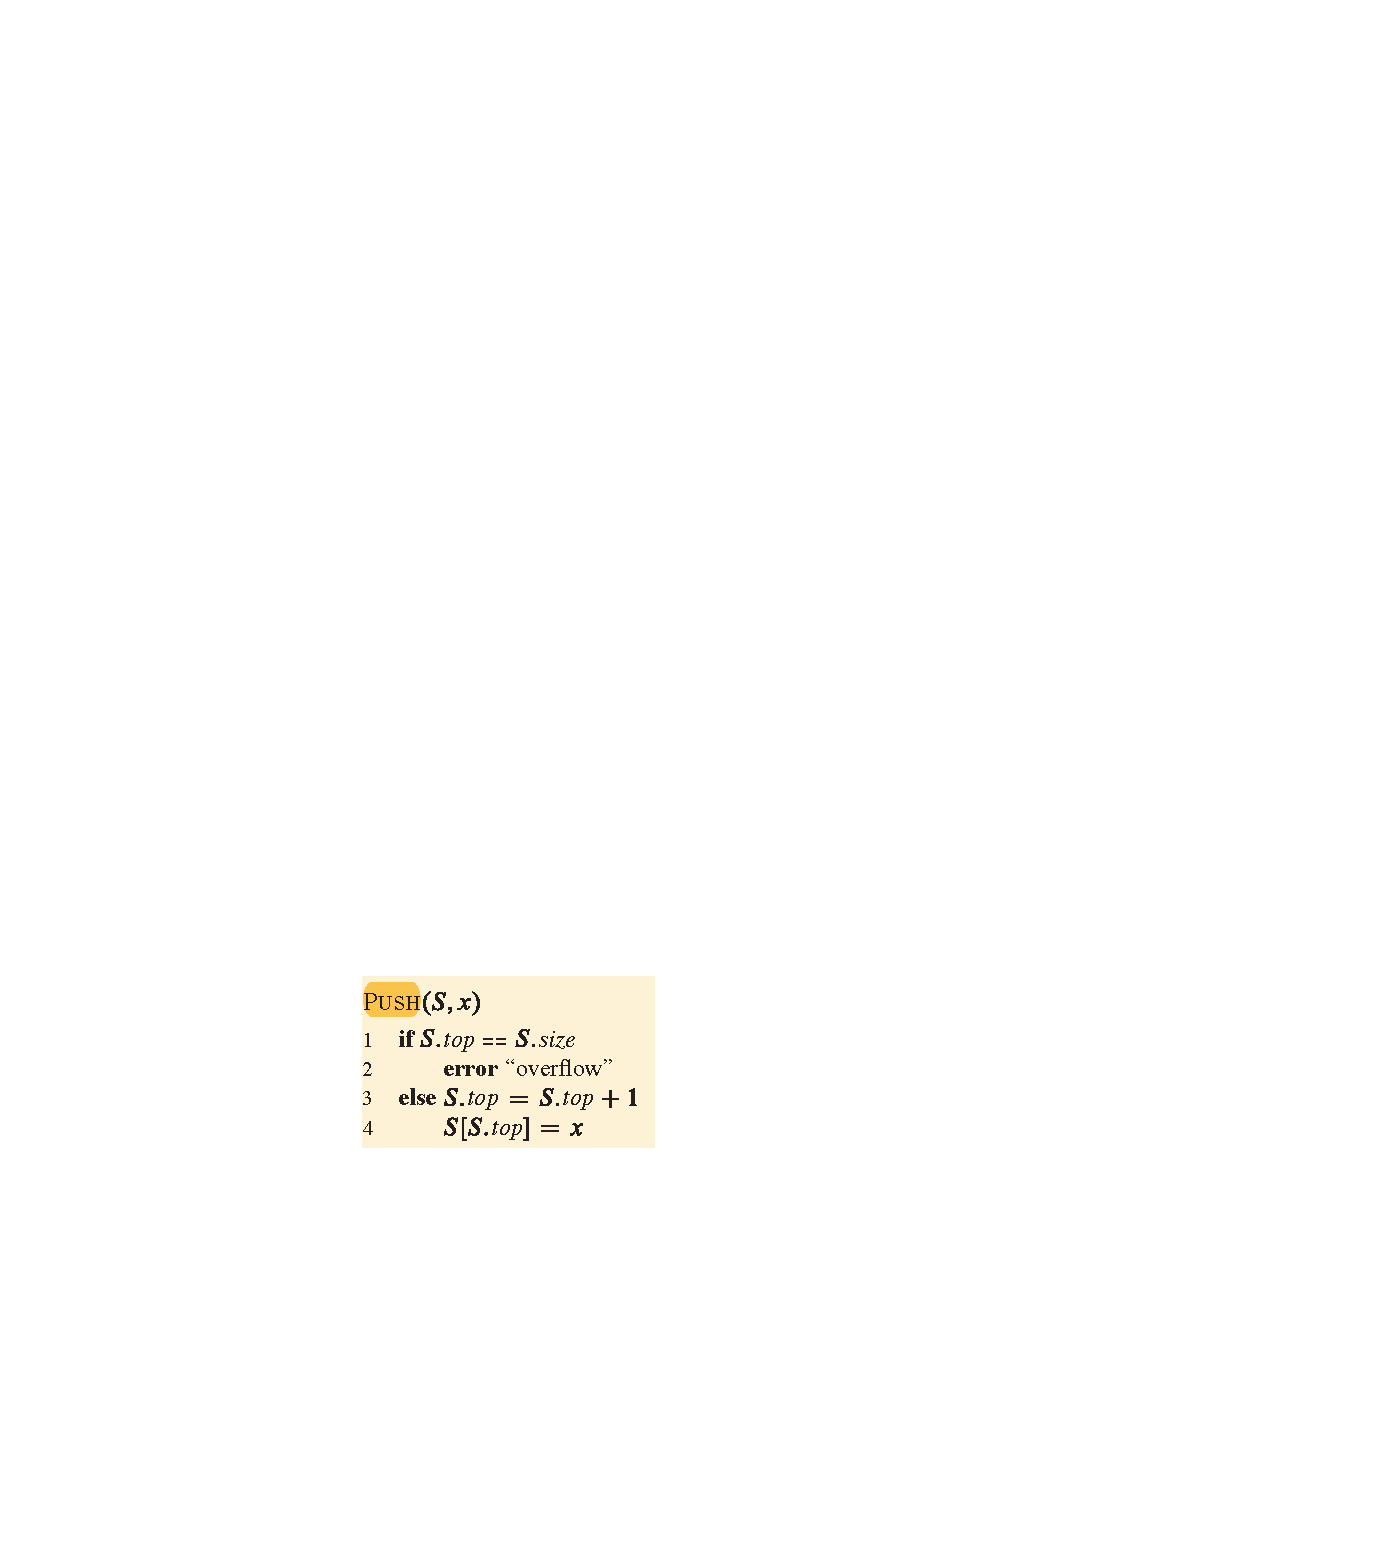
\includegraphics[width=.4\columnwidth]
			{fig-stack-push.pdf}
		\quad
		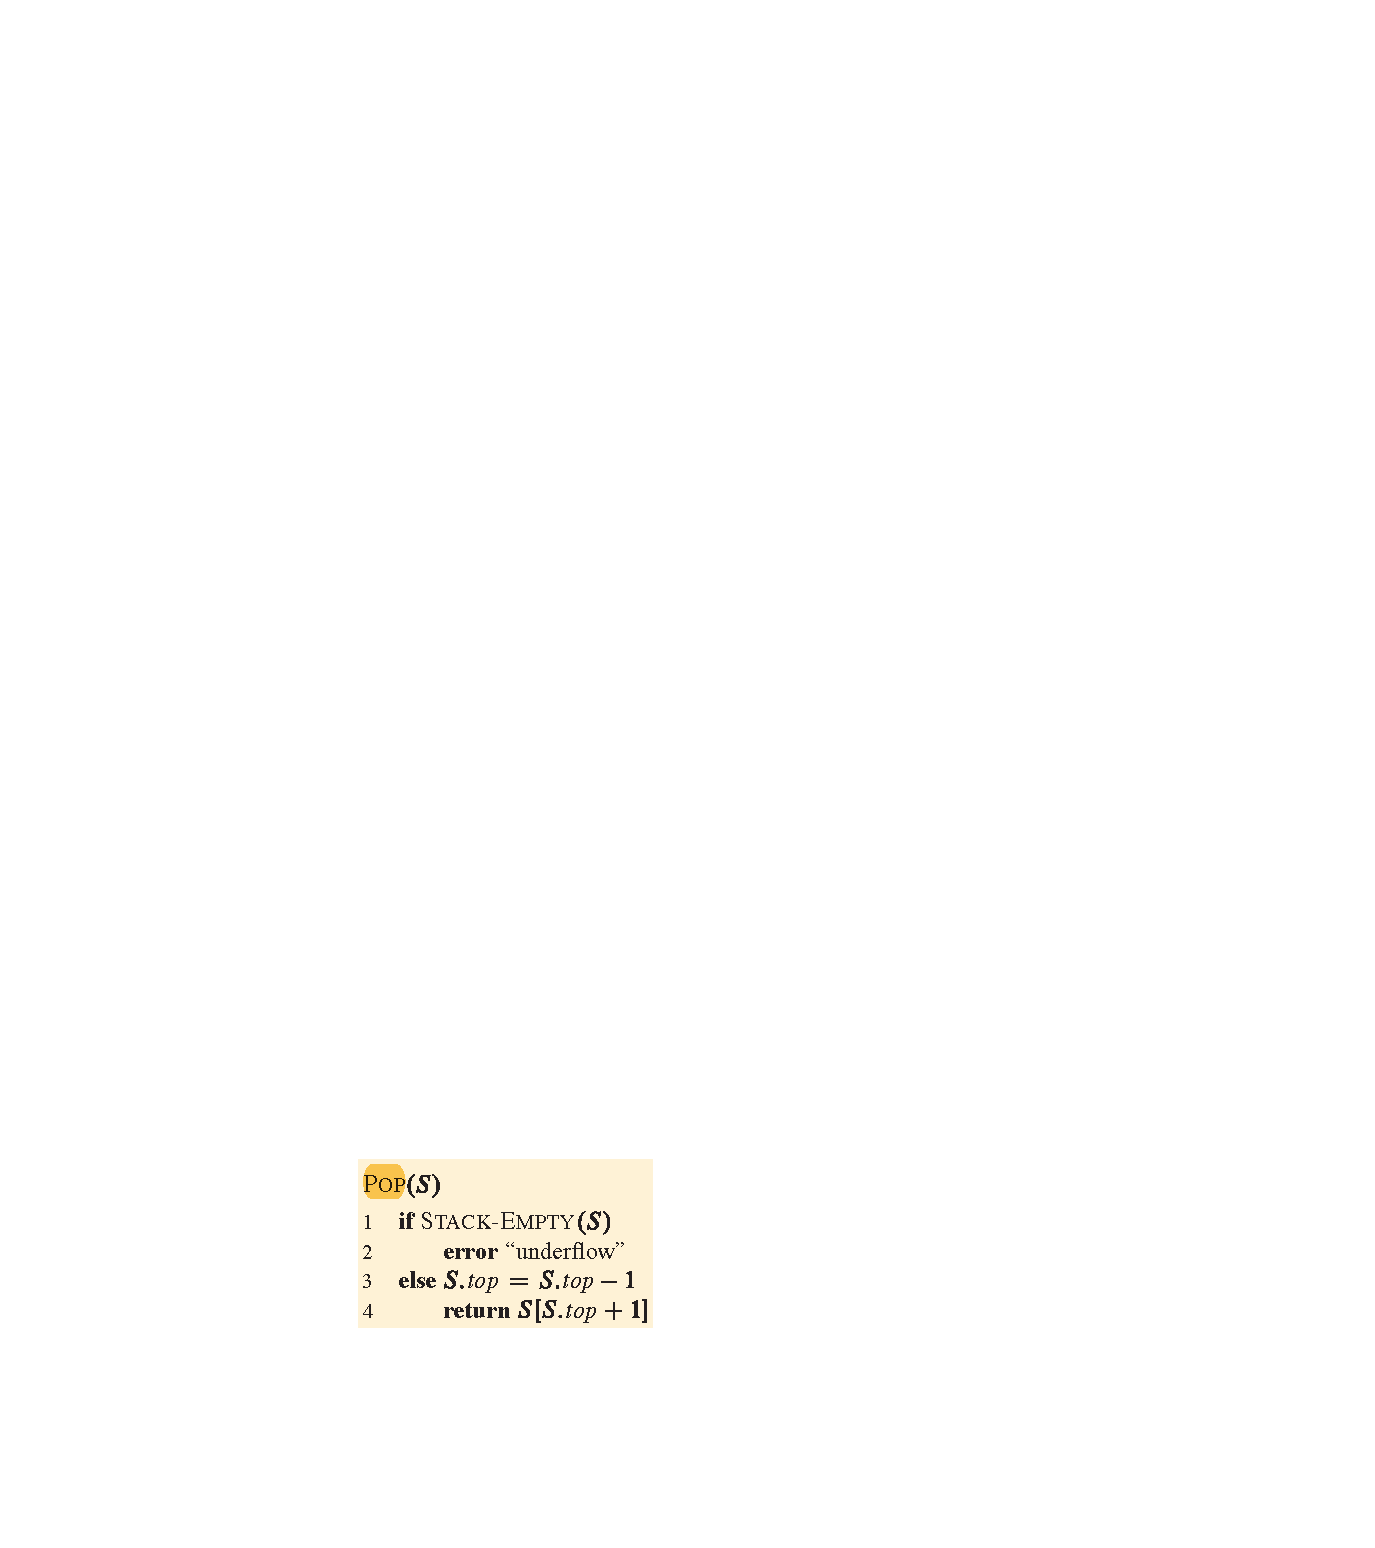
\includegraphics[width=.4\columnwidth]
			{fig-stack-pop.pdf}
		\\
		\vspace{0.2cm}	
		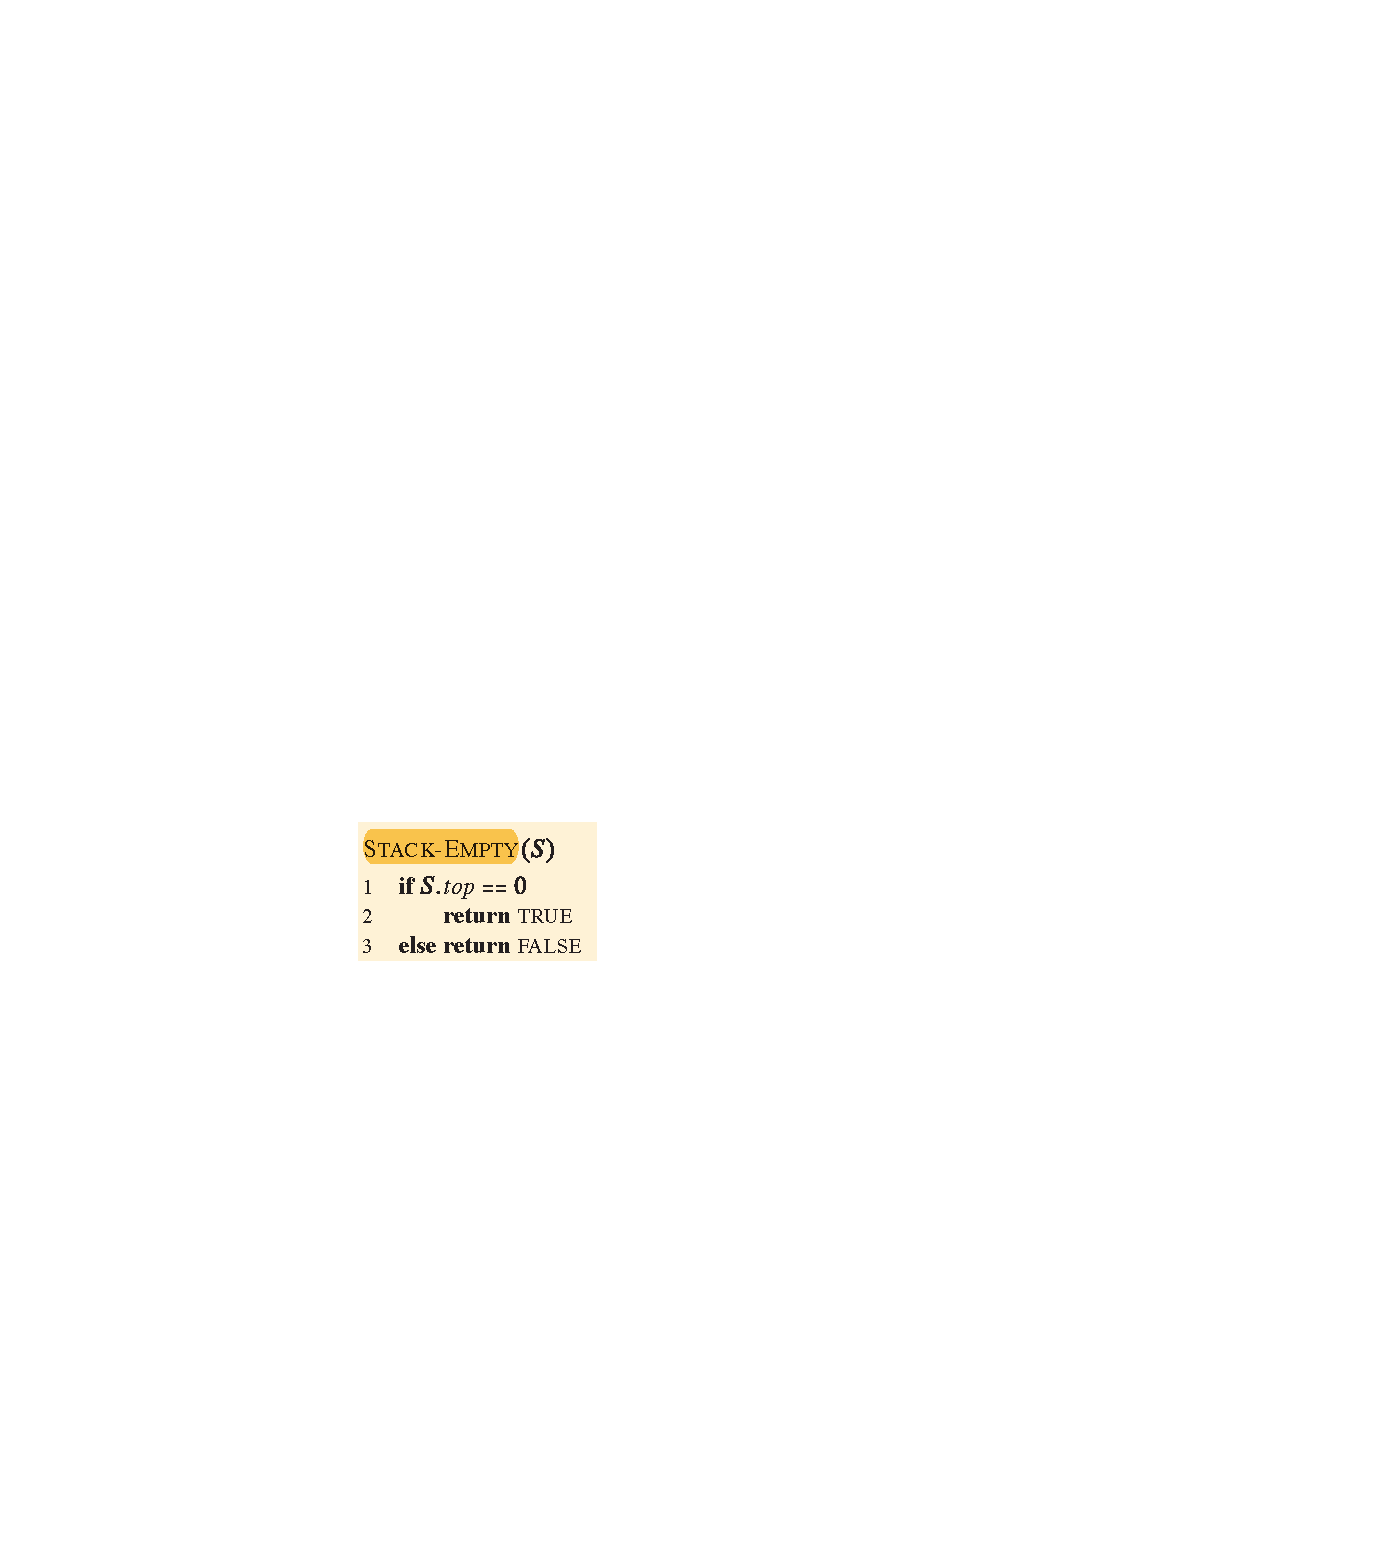
\includegraphics[width=.4\columnwidth]
			{fig-stack-empty.pdf}			
		\hCite{%
			source: CLRS~\cite{cormen2022introduction}
		}
		
		\hCite{%
			\cite{cormen2022introduction},%
			\cite{aho1974design},%
			\cite{horowitz1982fundamentals},%
			\cite{horstmann2016big}
		}
					
	\end{column} % ++++ A
	\begin{column}{.5\linewidth} % ++++ V

	\vspace{-1cm}
	    	\textbf{Array}\\
		%
		\begin{tikzpicture}
			\hStack{0}{4}{0}{A, , , }[0.5][0.5]
		\end{tikzpicture}\\
		%
		\begin{tikzpicture}
			\hStack{0}{4}{1}{A, B, , }[0.5][0.5]
		\end{tikzpicture}\\
		%
		\begin{tikzpicture}
			\hStack{0}{4}{2}{A, B, C, }[0.5][0.5]
		\end{tikzpicture}\\
		%
		\begin{tikzpicture}
			\hStack{0}{4}{1}{A, B, C, }[0.5][0.5]
		\end{tikzpicture}\\
		%
		\begin{tikzpicture}
			\hStack{0}{4}{0}{A, B, C, }[0.5][0.5]
		\end{tikzpicture}\\
		%
		\begin{tikzpicture}
			\hStack{0}{4}{1}{A, D, C, }[0.5][0.5]
		\end{tikzpicture}\\
		%
		\begin{tikzpicture}
			\hStack{0}{4}{2}{A, D, E, }[0.5][0.5]
		\end{tikzpicture}\\
		%
		\begin{tikzpicture}
			\hStack{0}{4}{3}{A, D, E, F}[0.5][0.5]
		\end{tikzpicture}\\
		%
		\begin{tikzpicture}
			\hStack{0}{4}{2}{A, D, E, F}[0.5][0.5]
		\end{tikzpicture}\\

	\end{column} % ++++ A
	\end{columns} % <<<<
\end{frame}
% ~~~~~~~~~~~~~~~~~~~~~~~~~~~~~~~~~~~~~~ A




% ~~~~~~~~~~~~~~~~~~~~~~~~~~~~~~~~~~~~~~ V
\hSection{Abstraction}{Abstract Data Types (ADT)}{}
% ~~~~~~~~~~~~~~~~~~~~~~~~~~~~~~~~~~~~~~ A




% ~~~~~~~~~~~~~~~~~~~~~~~~~~~~~~~~~~~~~~ V
\hSubsection{Abstraction-ADT}{Container}{}
% ~~~~~~~~~~~~~~~~~~~~~~~~~~~~~~~~~~~~~~ A




% ~~~~~~~~~~~~~~~~~~~~~~~~~~~~~~~~~~~~~~ V
\begin{frame}\frametitle{Abstraction-ADT: \hEmph{Container}}
	\begin{columns}[T] % >>>>
	\begin{column}{.5\linewidth} % ++++ V
	    	Container: contains items
		\begin{itemize}
			\item \hEmph{insert}(item)
			\item \hEmph{delete}(item)
			\item \hEmph{isIn}(item)
			\item \hEmph{isEmpty}()
			\item \hEmph{isFull}()
			\item \hEmph{size}()			
		\end{itemize}
	\end{column} % ++++ A
	\begin{column}{.5\linewidth} % ++++ V
		\begin{itemize}

			\item
			Insertion
			\begin{itemize}
				\item
				Order of is \hEmph{not} important
	
				\item
				Duplication is allowed
			\end{itemize}

			\item
			Deletion
			\begin{itemize}
				\item
				Any item can be deleted
			\end{itemize}
		\end{itemize}
	\end{column} % ++++ A
	\end{columns} % <<<<
\end{frame}
% ~~~~~~~~~~~~~~~~~~~~~~~~~~~~~~~~~~~~~~ A




% ~~~~~~~~~~~~~~~~~~~~~~~~~~~~~~~~~~~~~~ V
\hSubsection{Abstraction-ADT}{Set}{}
% ~~~~~~~~~~~~~~~~~~~~~~~~~~~~~~~~~~~~~~ A




% ~~~~~~~~~~~~~~~~~~~~~~~~~~~~~~~~~~~~~~ V
\begin{frame}\frametitle{Abstraction-ADT: \hEmph{Set}}
	\begin{columns}[T] % >>>>
	\begin{column}{.5\linewidth} % ++++ V
	    	Container: contains items
		\begin{itemize}
			\item insert(item)
			\item delete(item)
			\item isIn(item)
			\item isEmpty()
			\item isFull()
			\item size()			
		\end{itemize}
	\end{column} % ++++ A
	\begin{column}{.5\linewidth} % ++++ V
		\begin{itemize}

			\item
			Insertion
			\begin{itemize}
				\item
				Order of is \hEmph{not} important
	
				\item
				Duplication is  \hEmph{not} allowed
			\end{itemize}

			\item
			Deletion
			\begin{itemize}
				\item
				Any item can be deleted
			\end{itemize}
		\end{itemize}
	\end{column} % ++++ A
	\end{columns} % <<<<
\end{frame}
% ~~~~~~~~~~~~~~~~~~~~~~~~~~~~~~~~~~~~~~ A




% ~~~~~~~~~~~~~~~~~~~~~~~~~~~~~~~~~~~~~~ V
\hSubsection{Abstraction-ADT}{Stack}{}
% ~~~~~~~~~~~~~~~~~~~~~~~~~~~~~~~~~~~~~~ A




% ~~~~~~~~~~~~~~~~~~~~~~~~~~~~~~~~~~~~~~ V
\begin{frame}\frametitle{Abstraction-ADT: \hEmph{Stack}}
	\begin{columns}[T] % >>>>
	\begin{column}{.5\linewidth} % ++++ V
	    	Container: contains items
		\begin{itemize}
			\item \hEmph{push}(item) \sout{insert(item)}
			\item \hEmph{pop()} \sout{delete(item)}
			\item \sout{isIn(item)}
			\item \hEmph{isEmpty}()
			\item \hEmph{isFull}()
			\item \sout{size()}			
		\end{itemize}
	\end{column} % ++++ A
	\begin{column}{.5\linewidth} % ++++ V
		\begin{itemize}

			\item
			\hEmph{Last-In-First-Out} (\hEmph{LIFO})

			\item
			Insertion
			\begin{itemize}
				\item
				Order of is \hEmph{important} 
	
				\item
				Duplication is \hEmph{allowed}
			\end{itemize}

			\item
			Deletion
			\begin{itemize}
				\item
				\sout{Any item can be deleted}
				
				\item
				Only a \hEmph{specific} item can be deleted
			\end{itemize}
		\end{itemize}
	\end{column} % ++++ A
	\end{columns} % <<<<
\end{frame}
% ~~~~~~~~~~~~~~~~~~~~~~~~~~~~~~~~~~~~~~ A




% ~~~~~~~~~~~~~~~~~~~~~~~~~~~~~~~~~~~~~~ V
\hSection{Applications}{}{}
% ~~~~~~~~~~~~~~~~~~~~~~~~~~~~~~~~~~~~~~ A




% ~~~~~~~~~~~~~~~~~~~~~~~~~~~~~~~~~~~~~~ V
\hSubsection{Applications}{Balanced parentheses}{}
% ~~~~~~~~~~~~~~~~~~~~~~~~~~~~~~~~~~~~~~ A




% ~~~~~~~~~~~~~~~~~~~~~~~~~~~~~~~~~~~~~~ V
\begin{frame}\frametitle{Balanced Parentheses}
	\begin{columns}[T] % >>>>
	\begin{column}{.5\linewidth} % ++++ V
{\tiny 
\begin{algorithm}[H]
	\SetKwData{Stack}{\texttt{stack}}
	\SetKwData{Ch}{\texttt{ch}}
	\SetKwData{Cs}{\texttt{cs}}
	\KwData{algebraic expression}
	\KwResult{true if parentheses are balanced}
	\Begin{
		\ForEach {\Ch in expression from left to right} {
		
			\If {\Ch is an opening parenthesis} {
				push \Ch on the \Stack
			}\ElseIf {\Ch is a closing parenthesis} {
				\Cs $\leftarrow$ pop the \Stack \\
				\If {the opening \Cs and closing \Ch parentheses don’t match} {
					\Return FALSE 
				}
			}
		}
		\If {at the end the \Stack is empty} {
			\Return TRUE 
		} \Else {
			\Return FALSE
		}
	    
		\caption{{\footnotesize Balanced Parentheses}}
	}
\end{algorithm}
} % \tiny

\hCite{Horstmann~\cite{horstmann2016big}}

	\end{column} % ++++ A
	\begin{column}{.5\linewidth} % ++++ V
	
	\vspace{-1cm}
{\tiny
	expression: (~)~(~(~(~)~(~)~)~)\\
	\begin{center}
	\begin{tabular}{l l}
		\textbf{ch}
		&\textbf{stack}\\
		
		(
		&\begin{tikzpicture}
			\hStack{0}{4}{0}{``(''} [0.5][0.5]
		\end{tikzpicture}\\			
		
		)
		&\begin{tikzpicture}
			\hStack{0}{4}{-1}{} [0.5][0.5]
		\end{tikzpicture}\\			
		
		(
		&\begin{tikzpicture}
			\hStack{0}{4}{0}{``(''} [0.5][0.5]
		\end{tikzpicture}\\			
		
		(
		&\begin{tikzpicture}
			\hStack{0}{4}{1}{``('', ``(''} [0.5][0.5]
		\end{tikzpicture}\\			
		
		(
		&\begin{tikzpicture}
			\hStack{0}{4}{2}{``('', ``('', ``(''} [0.5][0.5]
		\end{tikzpicture}\\			
		
		)
		&\begin{tikzpicture}
			\hStack{0}{4}{1}{``('', ``(''} [0.5][0.5]
		\end{tikzpicture}\\			
		
		(
		&\begin{tikzpicture}
			\hStack{0}{4}{2}{``('', ``('', ``(''} [0.5][0.5]
		\end{tikzpicture}\\			
		
		)
		&\begin{tikzpicture}
			\hStack{0}{4}{1}{``('', ``(''} [0.5][0.5]
		\end{tikzpicture}\\			
		
		)
		&\begin{tikzpicture}
			\hStack{0}{4}{0}{``(''} [0.5][0.5]
		\end{tikzpicture}\\			
		
		)
		&\begin{tikzpicture}
			\hStack{0}{4}{-1}{} [0.5][0.5]
		\end{tikzpicture}
		{\small \hEmph{~~ Balanced}}\\			

	\end{tabular}
\end{center}
} % \tiny
	\end{column} % ++++ A
	\end{columns} % <<<<
\end{frame}
% ~~~~~~~~~~~~~~~~~~~~~~~~~~~~~~~~~~~~~~ A




%% ~~~~~~~~~~~~~~~~~~~~~~~~~~~~~~~~~~~~~~ V
%\begin{frame}\frametitle{Balanced Tags}
%	\lstset{
%		language=xml,
%		tabsize=3,
%		%frame=lines,
%%		caption=Test,
%		label=code:sample,
%		frame=shadowbox,
%		rulesepcolor=\color{gray},
%		xleftmargin=20pt,
%		framexleftmargin=15pt,
%		keywordstyle=\color{blue},
%		commentstyle=\color{darkgreen},
%		stringstyle=\color{red},
%%		numbers=left,
%%		numberstyle=\tiny,
%%		numbersep=5pt,
%		breaklines=true,
%		showstringspaces=false,
%		basicstyle=\tiny,
%		stringstyle=\color{blue},
%		emph={html,head,title,body,note,to,from,heading},emphstyle={\color{magenta}}
%	}
%	\begin{itemize}
%		
%		\item 
%		\hEmph{Arithmetic expressions}
%		\begin{itemize}			
%			\item 
%			$[a+b]*(c-d)$
%		\end{itemize}
%	
%		\item 
%		\hEmph{HTML tags}
%		\lstinputlisting{code-sample-html.html}
%		
%		\item 
%		\hEmph{XML tags}
%		\lstinputlisting{code-sample-xml.xml}
%	\end{itemize}
%
%\end{frame}
%% ~~~~~~~~~~~~~~~~~~~~~~~~~~~~~~~~~~~~~~ A




% ~~~~~~~~~~~~~~~~~~~~~~~~~~~~~~~~~~~~~~ V
\hSubsection{Applications}{Postfix Evaluation}{}
% ~~~~~~~~~~~~~~~~~~~~~~~~~~~~~~~~~~~~~~ A




% ~~~~~~~~~~~~~~~~~~~~~~~~~~~~~~~~~~~~~~ V
\begin{frame}\frametitle{Infix, Prefix, and Postfix (RPN) Notations}
% https://www.calcont.in/Conversion/infix_to_prefix
\begin{center}
\begin{tabular}{l l l}
	\textbf{infix notation} 
	&\textbf{prefix notation} 
	&\textbf{postfix notation}\\
	%
	{\tiny normal math expression} 
	&{\tiny operators followed by operands} 
	&{\tiny operands followed by operators}\\
	%
	$a + b$
	&$+ a~b$
	&$a~b +$\\
	%
	$a+b+c$
	&$+a + b~c$
	&$a~b + c +$\\
	%
	$a + b * c$
	&$+ a * b~c$
	&$a~b~c*+$\\
	%
	$(a + b) * c$
	&$*+a~b~c$
	&$a~b+c*$\\
	%
	$a+b*c/(e-f)$
	&$+a~/*b~c-e~f$
	&$a~b~c*e~f-/+$\\
	%
	~
	&~
	&	\hCite{
		\href
			{https://hp15c.com/web/hp15c.html}
			{HP-15 calculator online}~\cite{hp15online}
	}
\end{tabular}
\end{center}

	\vspace{1cm}
	Postfix notation is also called  
		\href
			{https://en.wikipedia.org/wiki/Reverse_Polish_notation}
			{\hEmph{Reverse Polish Notation (RPN)}}~\cite{wikipediaRPN}
	

	\hCite{%
		\href
			{https://www.openbookproject.net/books/pythonds/BasicDS/InfixPrefixandPostfixExpressions.html}
			{Infix, Prefix and Postfix Expressions}~\cite{pswadsPostfix}	
	}\\
	\hCite{%
		\href
			{https://www.web4college.com/converters/infix-to-postfix-prefix.php}
			{Infix to Postfix/Prefix converter}
	}

\end{frame}
% ~~~~~~~~~~~~~~~~~~~~~~~~~~~~~~~~~~~~~~ A




% ~~~~~~~~~~~~~~~~~~~~~~~~~~~~~~~~~~~~~~ V
\begin{frame}\frametitle{RPN Evaluation}
	\begin{columns}[T] % >>>>
	\begin{column}{.4\linewidth} % ++++ V
{\tiny 


% +++++++++++++++++++++++++++++++++++++++ V
%: -Alg. 
\begin{algorithm}[H]
	\SetKwData{Stack}{\texttt{stack}}
	\KwData{postfix expression}
	\KwResult{value of the expression}
	\Begin{
		\While {there is a token}{
			\If{an operator is read} {
				Pop two values off the \Stack\\
				Apply the operator to the two values \\
				Push the result back onto the \Stack
			} \ElseIf{a number is read} {
				Push it on the \Stack
			} 
		}
		Pop and display the result
	\caption{{\footnotesize RPN Evaluation}}
	}
\end{algorithm}
% +++++++++++++++++++++++++++++++++++++++ A

}

\hCite{Horstmann~\cite{horstmann2016big}}\\
\hCite{
	\href
		{https://hp15c.com/web/hp15c.html}
		{HP-15 calculator online}~\cite{hp15online}
}


	\end{column} % ++++ A
	\begin{column}{.4\linewidth} % ++++ V
	
		\vspace{-1cm}
		Use one stack\\
{\tiny
\begin{center}
	\begin{tabular}{l l}
		%
		\textbf{token}
		&\textbf{stack}\\
		%
		3
		&\begin{tikzpicture}
			\hStack{0}{5}{0}{3} [0.5][0.5]
		\end{tikzpicture}\\
		%
		4
		&\begin{tikzpicture}
			\hStack{0}{5}{1}{3, 4} [0.5][0.5]
		\end{tikzpicture}\\
		%
		+
		&\begin{tikzpicture}
			\hStack{0}{5}{0}{7} [0.5][0.5]
		\end{tikzpicture}\\
		%
		5
		&\begin{tikzpicture}
			\hStack{0}{5}{1}{7, 5} [0.5][0.5]
		\end{tikzpicture}\\
		%
		6
		&\begin{tikzpicture}
			\hStack{0}{5}{2}{7, 5, 6} [0.5][0.5]
		\end{tikzpicture}\\
		%
		-
		&\begin{tikzpicture}
			\hStack{0}{5}{1}{7, -1} [0.5][0.5]
		\end{tikzpicture}\\
		%
		*
		&\begin{tikzpicture}
			\hStack{0}{5}{0}{-7} [0.5][0.5]
		\end{tikzpicture}\\
		%
		~
		&\begin{tikzpicture}
			\hStack{0}{5}{-1}{} [0.5][0.5]
		\end{tikzpicture}
		~~~ {\small \hEmph{-7}}\\

	\end{tabular}
\end{center}
} % tiny
	\end{column} % ++++ A
	\begin{column}{.2\linewidth} % ++++ V
		\vspace{1cm}
		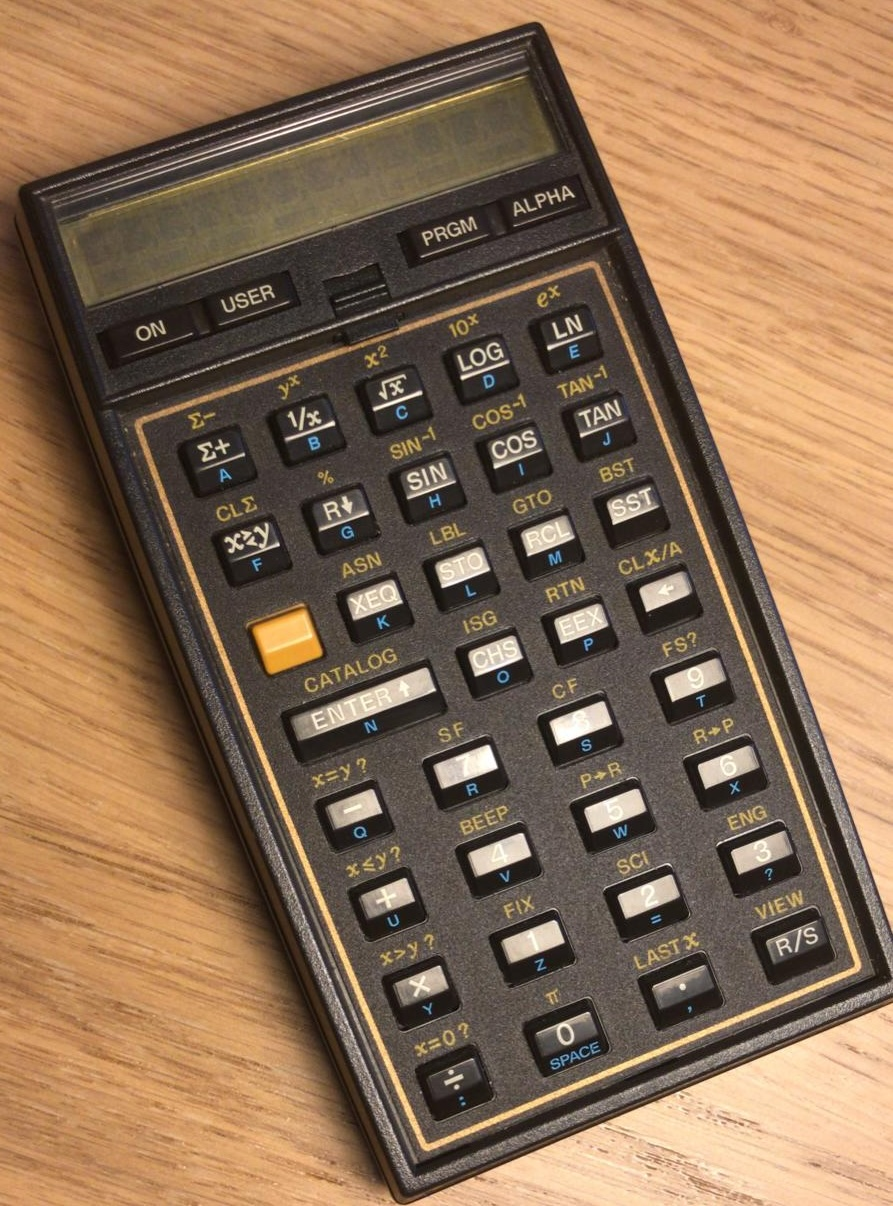
\includegraphics[width=\columnwidth]
			{fig-HP-41CV.jpg}
			{\tiny 
				HP-41CV,\\ 
				RPN Calculator,\\ 
				1979-1990\\
			}
	\end{column} % ++++ A
	\end{columns} % <<<<
\end{frame}
% ~~~~~~~~~~~~~~~~~~~~~~~~~~~~~~~~~~~~~~ A




%% ~~~~~~~~~~~~~~~~~~~~~~~~~~~~~~~~~~~~~~ V
%\begin{frame}\frametitle{RPN Evaluation}
%	\hCodeOutput{code-stack-RPN_Evaluator}[3.5][2.5]
%\end{frame}
%% ~~~~~~~~~~~~~~~~~~~~~~~~~~~~~~~~~~~~~~ A



% ~~~~~~~~~~~~~~~~~~~~~~~~~~~~~~~~~~~~~~ V
\hSubsection{Applications}{Infix to postfix conversion}{}
% ~~~~~~~~~~~~~~~~~~~~~~~~~~~~~~~~~~~~~~ A




% ~~~~~~~~~~~~~~~~~~~~~~~~~~~~~~~~~~~~~~ V
\begin{frame}\frametitle{Infix to postfix conversion}
	\begin{columns}[T] % >>>>
	\begin{column}{.5\linewidth} % ++++ V
	    	Use two stacks
		\begin{itemize}
			\item
			operator stack
			\item
			output stack
		\end{itemize}
	\end{column} % ++++ A
	\begin{column}{.7\linewidth} % ++++ V
	
			\vspace{-0.8cm}
{\small 
{\tt %mono space
\begin{center}
\begin{tabular}{|l|l|l|}
\hline
%\textbf{Input String} &\textbf{Output Stack} &\textbf{Operator Stack}\\
\textbf{Input } &\textbf{Stack} &\textbf{Stack}\\
\textbf{String} &\textbf{Output} &\textbf{Operator}\\
\hline
(f-e)/c*b+a & &(\\
(f-e)/c*b+a &f &(\\
(f-e)/c*b+a &f &(-\\
(f-e)/c*b+a &fe &(-\\
(f-e)/c*b+a &fe- &\\
(f-e)/c*b+a &fe- &/\\
(f-e)/c*b+a &fe-c &/\\
(f-e)/c*b+a &fe-c/ &*\\
(f-e)/c*b+a &fe-c/b &*\\
(f-e)/c*b+a &fe-c/b* &+\\
(f-e)/c*b+a &fe-c/b*a &+\\
(f-e)/c*b+a &fe-c/b*a+ &\\
\hline
\end{tabular}
\end{center}
}}

	\end{column} % ++++ A
	\end{columns} % <<<<
\end{frame}
% ~~~~~~~~~~~~~~~~~~~~~~~~~~~~~~~~~~~~~~ A



% ~~~~~~~~~~~~~~~~~~~~~~~~~~~~~~~~~~~~~~ V
\hSubsection{Applications}{Infix evaluation}{}
% ~~~~~~~~~~~~~~~~~~~~~~~~~~~~~~~~~~~~~~ A



% ~~~~~~~~~~~~~~~~~~~~~~~~~~~~~~~~~~~~~~ V
\begin{frame}\frametitle{Infix Evaluation}
	\begin{columns}[T] % >>>>
	\begin{column}{.5\linewidth} % ++++ V
{\tiny 
\begin{algorithm}[H]
	\SetKwData{StackOperand}{\texttt{stackOperand}}
	\SetKwData{StackOperator}{\texttt{stackOperator}}
	\SetKwData{Op}{\texttt{op}}
%    \KwData{infix algebraic expression}
%    \KwResult{value of the expression}
    \Begin{
 	\If{a number is read}
		 {Push it on the \StackOperand}
	\ElseIf{a ``(``  is read}
		{Push it on the \StackOperator}
	\ElseIf{operator \Op is read} {
		\While{the top of \StackOperator has a higher precedence than \Op}{
			Evaluate the top
		}
		Push \Op on \StackOperator
	}		
	\ElseIf {a ``)'' is read}{
		\While {the top of \StackOperator is not a ``(''}{
			Evaluate the top. 
		}
		Pop the ``(''
	}
	\ElseIf {there is no more input}{
		\While {the \StackOperator is not empty}{
			Evaluate the top
		}
	}
	Pop and display the result
    \caption{{\footnotesize Infix Evaluation}}
    }
\end{algorithm}
}

\hCite{Horstmann~\cite{horstmann2016big}}

	\end{column} % ++++ A
	\begin{column}{.5\linewidth} % ++++ V
	
	\vspace{-1.2cm}
\begin{center}
{\tiny
	expression: $(3+4)*(5-6)$\\
	
\begingroup
\setlength{\tabcolsep}{3pt}
\renewcommand{\arraystretch}{.2}
	\begin{tabular}{l l l}
		%
		\textbf{ch}
		&\textbf{stackOperand}
		&\textbf{stackOperator}\\
		%		
		(
		&\begin{tikzpicture}
			\hStack{0}{4}{-1}{} [0.5][0.4]
		\end{tikzpicture}
		&\begin{tikzpicture}
			\hStack{0}{4}{0}{``(''} [0.5][0.4]
		\end{tikzpicture}\\			
		%
		3
		&\begin{tikzpicture}
			\hStack{0}{4}{0}{3} [0.5][0.4]
		\end{tikzpicture}
		&\begin{tikzpicture}
			\hStack{0}{4}{0}{``(''} [0.5][0.4]
		\end{tikzpicture}\\	
		%
		+
		&\begin{tikzpicture}
			\hStack{0}{4}{0}{3} [0.5][0.4]
		\end{tikzpicture}
		&\begin{tikzpicture}
			\hStack{0}{4}{1}{``('', +} [0.5][0.4]
		\end{tikzpicture}\\	
		%
		4
		&\begin{tikzpicture}
			\hStack{0}{4}{1}{3, 4} [0.5][0.4]
		\end{tikzpicture}
		&\begin{tikzpicture}
			\hStack{0}{4}{1}{``('', +} [0.5][0.4]
		\end{tikzpicture}\\	
		%
		)
		&\begin{tikzpicture}
			\hStack{0}{4}{0}{7} [0.5][0.4]
		\end{tikzpicture}
		&\begin{tikzpicture}
			\hStack{0}{4}{-1}{} [0.5][0.4]
		\end{tikzpicture}\\	
		%
		*
		&\begin{tikzpicture}
			\hStack{0}{4}{0}{7} [0.5][0.4]
		\end{tikzpicture}
		&\begin{tikzpicture}
			\hStack{0}{4}{0}{*} [0.5][0.4]
		\end{tikzpicture}\\	
		%
		(
		&\begin{tikzpicture}
			\hStack{0}{4}{0}{7} [0.5][0.4]
		\end{tikzpicture}
		&\begin{tikzpicture}
			\hStack{0}{4}{1}{*, ``(''} [0.5][0.4]
		\end{tikzpicture}\\	
		%
		5
		&\begin{tikzpicture}
			\hStack{0}{4}{1}{7, 5} [0.5][0.4]
		\end{tikzpicture}
		&\begin{tikzpicture}
			\hStack{0}{4}{1}{*, ``(''} [0.5][0.4]
		\end{tikzpicture}\\	
		%
		$-$
		&\begin{tikzpicture}
			\hStack{0}{4}{1}{7, 5} [0.5][0.4]
		\end{tikzpicture}
		&\begin{tikzpicture}
			\hStack{0}{4}{2}{*, ``('', $-$} [0.5][0.4]
		\end{tikzpicture}\\
		%
		6
		&\begin{tikzpicture}
			\hStack{0}{4}{2}{7, 5, 6} [0.5][0.4]
		\end{tikzpicture}
		&\begin{tikzpicture}
			\hStack{0}{4}{2}{*, ``('', $-$} [0.5][0.4]
		\end{tikzpicture}\\	
		%
		)
		&\begin{tikzpicture}
			\hStack{0}{4}{1}{7, $-1$} [0.5][0.4]
		\end{tikzpicture}
		&\begin{tikzpicture}
			\hStack{0}{4}{0}{*} [0.5][0.4]
		\end{tikzpicture}\\	
		%
		~
		&\begin{tikzpicture}
			\hStack{0}{4}{0}{-7} [0.5][0.4]
		\end{tikzpicture}
		&\begin{tikzpicture}
			\hStack{0}{4}{-1}{} [0.5][0.4]
		\end{tikzpicture}\\	
		%
		~
		&\begin{tikzpicture}
			\hStack{0}{4}{-1}{} [0.5][0.4]
		\end{tikzpicture}
		&\begin{tikzpicture}
			\hStack{0}{4}{-1}{} [0.5][0.4]
		\end{tikzpicture}~~~
		\hEmph{{\small -7}}\\
		
	\end{tabular}
	\endgroup

}
\end{center}
	\end{column} % ++++ A
	\end{columns} % <<<<
\end{frame}
% ~~~~~~~~~~~~~~~~~~~~~~~~~~~~~~~~~~~~~~ A




% ~~~~~~~~~~~~~~~~~~~~~~~~~~~~~~~~~~~~~~ V
\hSubsection{Applications}{Backtracking}{}
% ~~~~~~~~~~~~~~~~~~~~~~~~~~~~~~~~~~~~~~ A




% ~~~~~~~~~~~~~~~~~~~~~~~~~~~~~~~~~~~~~~ V
\begin{frame}\frametitle{Decision Tree}
	\begin{columns}[T] % >>>>
	\begin{column}{.5\linewidth} % ++++ V
{\footnotesize  
\begin{itemize}
	
	\item 
	At a decision point, select one path, push the unselected paths to stack.
	
	\item 
	If a path unsuccessfully ends, pop the stack for a new path.
	
	\item 
	Keep doing as long as there is untested path in the stack.
	
\end{itemize}
}

	
\begin{tikzpicture} [level distance=10mm,
every node/.style={fill=red!25,circle,inner sep=1pt},
level 1/.style={sibling distance=20mm,nodes={fill=red!25}}, 
level 2/.style={sibling distance=10mm,nodes={fill=red!25}}, 
level 3/.style={sibling distance=5mm,nodes={fill=red!25}}]
	\node {1}
	child {
		node {2}
		child {
			node {4}
			child {
				node {8}
			}
			child[missing]
		}
		child {
			node {5}
			child {
				node {10}
			}
			child[missing]
		}
	}
	child {
		node {3}
		child {
			node {6}
			child[missing]
			child {
				node {13}
			}
		}
		child {
			node {7}
		}
	};
\end{tikzpicture}
	\end{column} % ++++ A
	\begin{column}{.5\linewidth} % ++++ V

\vspace{-1cm}
{\tiny
\begin{center}
%	expression: (~)~(~(~(~)~(~)~)~)\\
	\begin{tabular}{l l}
		\textbf{node}
		&\textbf{stack}\\
		
		1
		&\begin{tikzpicture}
			\hStack{0}{4}{-1}{} [0.5][0.5]
		\end{tikzpicture}\\			
		
		2
		&\begin{tikzpicture}
			\hStack{0}{4}{0}{3} [0.5][0.5]
		\end{tikzpicture}\\			
		
		4
		&\begin{tikzpicture}
			\hStack{0}{4}{1}{3, 5} [0.5][0.5]
		\end{tikzpicture}\\			
		
		8
		&\begin{tikzpicture}
			\hStack{0}{4}{1}{3, 5} [0.5][0.5]
		\end{tikzpicture}\\			
		% leaf
		
		5
		&\begin{tikzpicture}
			\hStack{0}{4}{0}{3} [0.5][0.5]
		\end{tikzpicture}\\			
		
		10
		&\begin{tikzpicture}
			\hStack{0}{4}{0}{3} [0.5][0.5]
		\end{tikzpicture}\\			
		% leaf
		
		3
		&\begin{tikzpicture}
			\hStack{0}{4}{-1}{} [0.5][0.5]
		\end{tikzpicture}\\			
		
		6
		&\begin{tikzpicture}
			\hStack{0}{4}{0}{7} [0.5][0.5]
		\end{tikzpicture}\\			
		
		13
		&\begin{tikzpicture}
			\hStack{0}{4}{0}{7} [0.5][0.5]
		\end{tikzpicture}\\			
		% leaf
		
		7
		&\begin{tikzpicture}
			\hStack{0}{4}{-1}{} [0.5][0.5]
		\end{tikzpicture}\\			

	\end{tabular}
\end{center}
} % \tiny
	\end{column} % ++++ A
	\end{columns} % <<<<
\end{frame}
% ~~~~~~~~~~~~~~~~~~~~~~~~~~~~~~~~~~~~~~ A




% ~~~~~~~~~~~~~~~~~~~~~~~~~~~~~~~~~~~~~~ V
\begin{frame}\frametitle{Web resources}
	\begin{itemize}

		\item 
		Problem Solving with Algorithms and Data Structures using Python
		\begin{itemize}
			
			\item 
			Home~\cite{pswads}
		
			\item 
			Infix, Prefix and Postfix Expressions~\cite{pswadsPostfix}
			
			\item
			What is a Stack~\cite{pswadsStack} 
			
		\end{itemize}

		\item 
		The Java Tutorials by Oracle
		\begin{itemize}
			
			\item 
			Home~\cite{TheJavaTutorials}
			
			\item
			Arrays~\cite{TheJavaTutorialsArray}
			
			\item
			Generics~\cite{TheJavaTutorialsGenerics}
			
		\end{itemize}
		
		\item
		HP Calculators (An RPN Calculator)
		\begin{itemize}
			
			\item 
			\hCite{
				\href
					{https://hp15c.com/web/hp15c.html}
					{HP-15 calculator online}~\cite{hp15online}
			}
		\end{itemize}
	\end{itemize}
\end{frame}
% ~~~~~~~~~~~~~~~~~~~~~~~~~~~~~~~~~~~~~~ A



% ~~~~~~~~~~~~~~~~~~~~~~~~~~~~~~~~~~~~~~ V References bib
\begin{frame}[allowframebreaks]\frametitle{References}
	\setbeamertemplate{bibliography item}[text] % sets numbers in references
%	\bibliographystyle{abbrv}
%	\bibliographystyle{apalike}
%	\bibliographystyle{ieeetr}
	\bibliographystyle{IEEEtran}
	%
	\tiny\bibliography{../hbcommon/bingol-DataStructures} % bib file
	
\end{frame}
% ~~~~~~~~~~~~~~~~~~~~~~~~~~~~~~~~~~~~~~ A

% ~~~~~~~~~~~~~~~~~~~~~~~~~~~~~~~~~~~~~~~ 
\end{document}
